%license:BSD-3-Clause
%copyright-holders:Michele Maione
%============================================================
%
%	Piattaforma di cloud gaming per giochi arcade
%
%============================================================

\chapter{Introduzione}
\label{cap:Introduzione}

Il capitolo che apre questa tesi fa un'introduzione sulla nascita dei videogiochi, i ricavi globali dell'industria videoludica, il cloud gaming e i servizi presenti sul mercato.

\section{Nascita dei videogiochi}

Nel 1952 nei laboratori dell'Università di Cambridge, come esempio a corredo di una tesi di dottorato, fu creato OXO, la trasposizione del tris come gioco per computer. OXO è considerato tecnicamente il primo videogioco. Nel 1958 un professore di fisica del Brookhaven National Laboratory creò un gioco, Tennis for Two, che aveva il compito di simulare le leggi fisiche relative ad una partita di tennis, lo strumento utilizzato era un oscilloscopio.

Nel 1961, sei giovani scienziati del Massachusetts Institute of Technology su un PDP-1\footnote{PDP-1: Programmed Data Processor-1, era un computer della Digital Equipment Corporation del 1959.} crearono il primo videogioco a scopo di intrattenimento: Spacewar!.

Due mesi dopo due ingegneri elettrici, N. Bushnell e T. Dabney, terminarono la loro versione di Spacewar! su larga scala (1.500 copie), ma il gioco non ebbe un grande successo a causa dell'elevata difficoltà. Bushnell, dopo l'esperimento non particolarmente riuscito, decise però di insistere nel settore dando così vita alla società Atari. Il primo gioco arcade di Atari fu il primo grande successo del settore: Pong. Pubblicato alla fine del 1972, è un gioco che riproduce approssimativamente la meccanica del ping pong. Atari vendette 19.000 cabinati di Pong e presto molte altre società seguirono l'esempio. Alla fine del decennio iniziò l'epoca d'oro dei videogiochi arcade.

I videogiochi sono un mezzo di intrattenimento unico che combina le diverse forme d'arte, quali musica, narrativa e animazione, all'interattività. Ed è proprio questa caratteristica, l'interattività, che permette loro di esercitare un potenziale d'immersione e attrazione che altri media non hanno. Sono ormai diventati un fenomeno culturale di massa con centinaia di milioni di persone che giocano regolarmente ogni giorno, il che li rende un attore dominante nel settore dell'intrattenimento, settore in continua crescita che non ha mai subito interruzioni nel corso degli anni come mostrato in Fig. \ref{fig:valore_commerciale_giochi_globale}. Negli ultimi vent'anni l'importanza economica dei videogiochi arcade è notevolmente diminuita\footnote{Giappone, Cina e Corea mantengono una forte industria arcade ai giorni nostri.} (in viola nella figura) a favore dei videogiochi per personal computer, console e più recentemente per mobile.

\begin{figure}[H]
	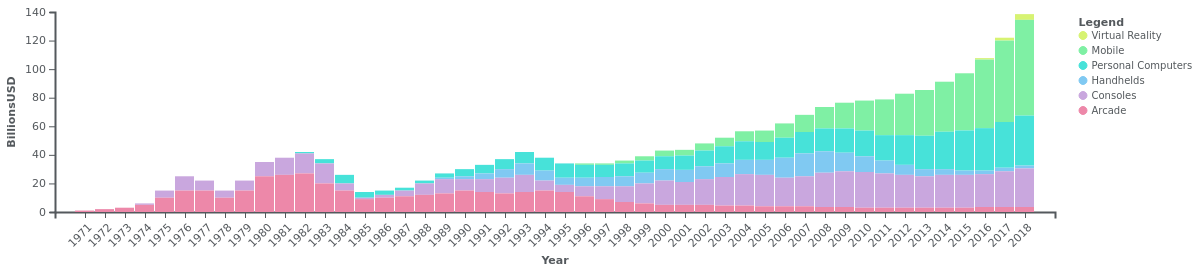
\includegraphics[width=\linewidth]{immagini/valore_commerciale_giochi_globale.png}
	\caption{Ricavi globali dell'industria dei videogiochi dal 1971 al 2018 (non adeguati all'inflazione). Fonte: wikipedia.org}
	\label{fig:valore_commerciale_giochi_globale}
\end{figure}

%\begin{figure}[H]
%	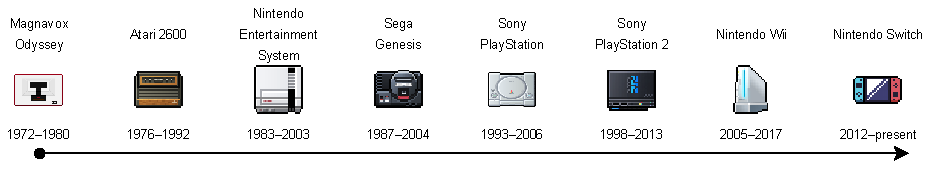
\includegraphics[width=\linewidth]{immagini/consoles_history}
%	\caption{Console iconiche, fino alla generazione otto}
%	\label{fig:consoles_history}
%\end{figure}

\section{Cloud gaming}
Il cloud gaming è un tipo di servizio online che funziona in modo simile al desktop remoto e al video on demand. I videogiochi vengono archiviati ed eseguiti in remoto, audio e video vengono trasmessi in streaming come un film sul dispositivo dell'utente, tramite un client. Il client gestisce gli input del giocatore, che vengono inviati al server ed eseguiti nel gioco.

Questo tipo di approccio offre molti vantaggi, tra cui: rende il gioco facilmente accessibile senza doverlo scaricare e installare localmente, è compatibile con computer e smartphone e anche con smart TV se utilizzato con un gamepad WiFi. Diversi servizi possono offrire alcune funzionalità aggiuntive per sfruttare al meglio questo modello, uno spettatore può unirsi alla sessione di un giocatore e assumere temporaneamente il controllo del gioco, se autorizzato dal giocatore stesso. Inoltre risolve definitivamente un problema che esiste dai tempi delle audiocassette e dei floppy disk: la pirateria. Il rapido sviluppo delle reti a banda larga e il continuo calo dei costi di abbonamento hanno reso questo metodo, oggi, una realtà.

Il più grande problema del cloud gaming era ed è ancora la latenza. Le fasi di un videogioco sono: ricezione input, esecuzione, rendering, display; mentre nel caso del cloud gaming abbiamo: ricezione input, invio input tramite rete, esecuzione, rendering, codifica, invio codifica tramite rete, decodifica, display. Un leggero ritardo in un filmato su internet o in una videochiamata molto probabilmente passa inosservato, ma durante una partita la latenza può rendere il gioco ingiocabile, una tempistica di esempio è visibile in Fig. \ref{fig:latenzaCloudGaming}.

\begin{figure}[H]
	\includegraphics[width=\linewidth]{immagini/latenzaCloudGaming.png}
	\caption{Latenza del videogioco: locale vs cloud gaming. Fonte: shadow.tech/blog/news/roadmap-cloud-gaming-without-latency}
	\label{fig:latenzaCloudGaming}
\end{figure}

\subsubsection{La nascita del cloud gaming}
Una delle prime piattaforme di cloud gaming è stata OnLive di OL2, presentato alla GDC\footnote{GDC: Game Developers Conference, una conferenza annuale per gli sviluppatori di videogiochi.} 2009 e poi lanciato sul mercato nel giugno 2010. I giocatori potevano acquistare giochi sulla piattaforma o giocare quelli precedentemente acquistati su Steam\footnote{Steam è un servizio di distribuzione digitale di videogiochi della società Valve.}.

Nel 2012, Gaikai ha inaugurato il suo omonimo servizio di cloud gaming, la società si è concentrata principalmente sull'utilizzo del cloud gaming come forma di pubblicità online per i videogiochi, dove gli utenti avrebbero avuto la possibilità di accedere alle demo dei videogiochi sponsorizzati.

OnLive e Gaikai sono stati acquisiti da Sony e le loro risorse sono state utilizzate come base per il servizio di cloud gaming noto come Playstation Now.

Nel 2013, Nvidia ha introdotto GeForce Now, un servizio di cloud gaming integrato nel suo dispositivo Shield TV\footnote{Nvidia Shield TV è un lettore multimediale digitale basato su Android.}. Nel 2017, la società ha iniziato a espandere il proprio servizio su PC, includendo il supporto per l'importazione della libreria giochi Steam.

Nel maggio 2018, Electronic Arts (EA) ha acquistato alcune risorse di cloud gaming da GameFly, e successivamente annunciò Project Atlas, un piattaforma di cloud gaming che in più esplorava l'integrazione di intelligenza artificiale e apprendimento automatico, rendendo la piattaforma dinamica, social e multipiattaforma.

Microsoft all'E3\footnote{E3: Electronic Entertainment Expo, un evento commerciale per l'industria dei videogiochi.} del 2018 ha annunciato la sua piattaforma Xbox Cloud Gaming.

Alla GDC 2019, Google ha annunciato ufficialmente il suo servizio di cloud gaming Stadia, in uscita per novembre dello stesso anno.

A settembre 2020, un nuovo servizio chiamato Luna è stato annunciato da Amazon\cite{Cloud_gaming_history}.

\subsubsection{Il caso Apple}
Apple aveva cercato di bloccare le app di cloud gaming sull'App Store a metà del 2020, ma a settembre 2020 decise di consentire il cloud gaming con alcune restrizioni: che i giochi offerti nel servizio dovessero essere scaricati direttamente dall'App Store, non da un'app all-in-one. I produttori di app sono autorizzati a rilasciare una cosiddetta "app catalogo" che si collega ad altri giochi nel servizio, ma ogni gioco dovrà essere una singola app e tutti i giochi e le "app catalogo" devono offrire l'acquisto solo tramite il sistema di elaborazione dei pagamenti "in‑app purchases", in base al quale Apple di solito prende il 30\% delle entrate\cite{Apple_controversy}.

\subsubsection{Cloud gaming market}
Secondo la ricerca di Newzoo sull'industria dei videogiochi, nel 2020 sono stati generati quasi \$585 milioni di entrate dal mercato del cloud gaming e si prevede una crescita fino a \$4,8 miliardi entro il 2023, se non maggiore. Per questo sono entrate nel mercato anche aziende che non sono produttori di videogiochi, come Google e Amazon.

\begin{figure}[H]
	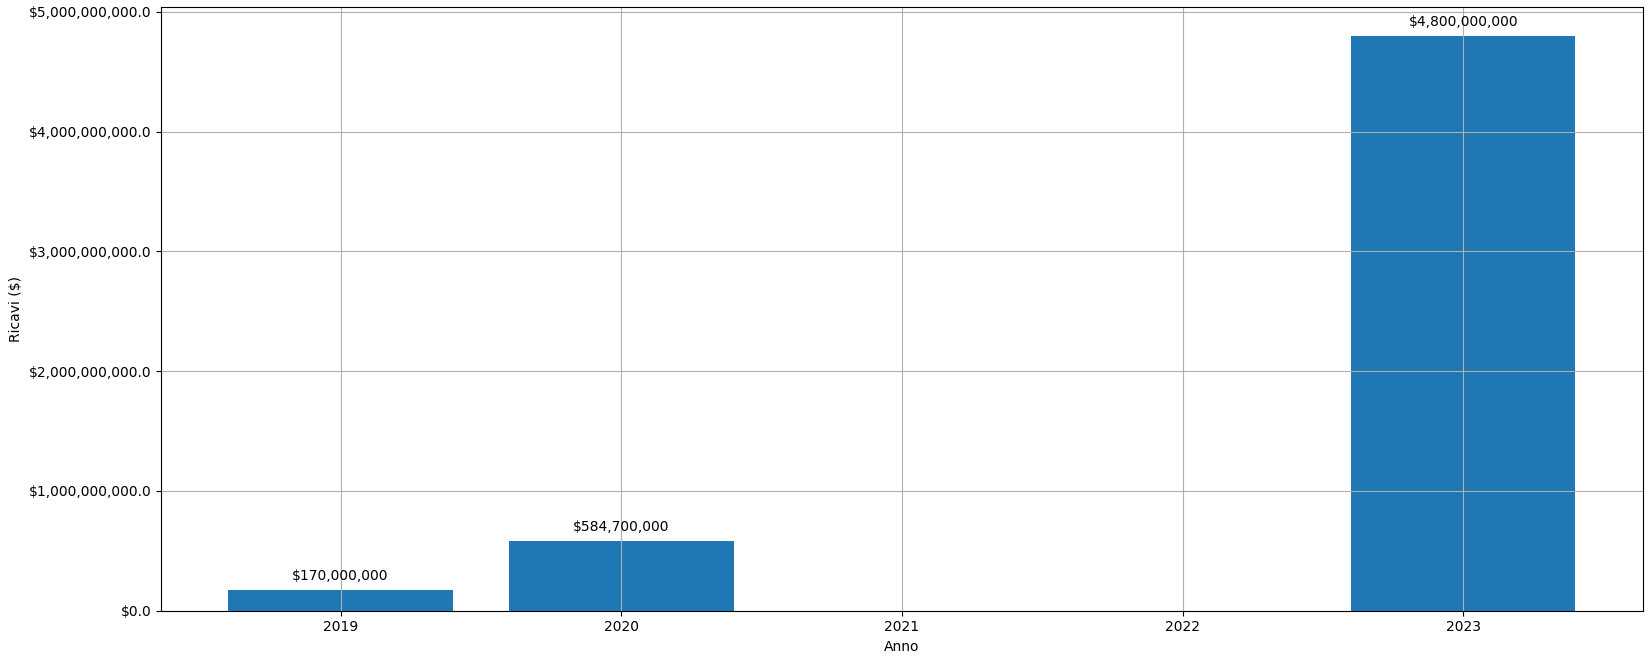
\includegraphics[width=\linewidth]{immagini/Newzoo_Cloud_Gaming_Revenues}
	\caption{Previsioni per il mercato globale del cloud gaming (in dollari americani). Fonte: newzoo.com/global-cloud-gaming-report}
	\label{fig:Newzoo_Cloud_Gaming_Revenues_Sept_2020}
\end{figure}

Vediamo l'attuale panorama del cloud gaming.

\subsection{Utomik}
La piattaforma Utomik è stata lanciata commercialmente nel 2008 e da allora è in servizio. I giochi per essere riprodotti in un browser richiedono il plug-in proprietario Utomik Player. La piattaforma offre un SDK, plug-in e servizi online per creare, avviare, mantenere e monitorare i giochi pubblicati\cite{Utomik}.

\subsection{Microsoft - Xbox Cloud Gaming}
Microsoft ha anticipato Xbox Cloud Gaming all'E3 2018. La piattaforma è disponibile per gli abbonati a Xbox Game Pass Ultimate da settembre 2020 ed offre sia la libreria esistente di giochi per Xbox che per Xbox Series X. Il servizio è progettato per funzionare con gli smartphone (attualmente solo Android), con controlli touchscreen o usando un controller Xbox tramite Bluetooth\cite{Xbox_Game_Pass_cloud_gaming}.

\subsection{Electronic Arts - Project Atlas}
A maggio 2018 Electronic Arts ha svelato la sua piattaforma di cloud gaming chiamata Project Atlas, che mira a rendere disponibili numerosi titoli e a fornire un'esperienza di gioco mai provata prima grazie al supporto dell'intelligenza artificiale. La piattaforma mira ad offrire un'esperienza di gioco composta da universi realmente viventi, che cambiano con il passare del tempo, con l'interazione con altri giocatori e sotto l'influenza del mondo esterno. In questi processi, il supporto dell'intelligenza artificiale e l'apprendimento delle abitudini e delle preferenze dei giocatori giocherebbero un ruolo fondamentale. Offre anche un client di gioco dinamico, che consente agli utenti di riprodurre in streaming un titolo mentre attendono il completamento del download sul proprio dispositivo\cite{Project_Atlas}.

\subsection{Nvidia - GeForce Now}
GeForce Now è il servizio di cloud gaming di Nvidia lanciato in beta a gennaio 2017 e ufficialmente a febbraio 2020. GeForce Now consente agli utenti di accedere da remoto (tramite streaming) a un computer virtuale, dove possono installare i giochi acquistati su Steam, Ubisoft Connect\footnote{Ubisoft Connect è un servizio di distribuzione digitale della società Ubisoft.} o Epic Games Store\footnote{Epic Games Store è un negozio di videogiochi digitali gestito da Epic Games.}. Il servizio può essere utilizzato su Windows, macOS, iOS, Android o Nvidia Shield TV\cite{GeForce_Now}.

\subsection{Sony - PlayStation Now}
PlayStation Now è un servizio di cloud gaming basato sulla tecnologia cloud di Gaikai utilizzando Microsoft Azure. È stato presentato durante il CES\footnote{CES: Consumer Electronics Show, un evento annuale che ospita presentazioni di nuovi prodotti e tecnologie nel settore dell'elettronica di consumo.} 2014. È disponibile da gennaio 2015 in Nord America, da settembre in Giappone e Regno Unito ed ha iniziato ad operare in Europa gradualmente da agosto 2017 a marzo 2019. La piattaforma consente all'utente di giocare ai titoli PlayStation (attualmente dal catalogo giochi della PS2, PS3 e PS4) su PS4, PS5 e Windows\cite{PlayStation_Now}.

\subsection{Google - Stadia}
Stadia è una piattaforma di cloud gaming rilasciata a novembre 2019, ma è disponibile solo in Europa e negli Stati Uniti. Sulla piattaforma l'utente può acquistare giochi o iscriversi al servizio per accedere al catalogo giochi. Google ha creato il controller Stadia che si connette tramite WiFi direttamente al servizio e rende possibile giocare su una TV (installando l'app o utilizzando un Chromecast\footnote{Google Chromecast è un lettore multimediale digitale per contenuti audiovisivi in streaming su Internet}). Invece sul computer tramite il browser Chrome si può giocare con mouse e tastiera o controller. Per quanto riguarda il mobile è disponibile un'app che supporta i controlli touch screen e i gamepad Bluetooth. La piattaforma offre alcune funzionalità interessanti come: live streaming su YouTube del proprio gameplay; Crowd Play che consente agli spettatori di unirsi ai giochi multiplayer che stanno guardando; Stream Connect che consente all'utente di condividere la schermata di gioco con altri giocatori nello stesso gioco; "Condivisione dello stato" che consente ai giocatori di condividere il proprio stato di salvataggio\cite{Google_Stadia}.

\subsection{Amazon - Luna}
Luna è stata annunciata a settembre 2020, con "accesso anticipato" disponibile per gli abbonati su invito a partire da ottobre 2020. Il catalogo giochi proposto consta di 100 giochi. La piattaforma è ovviamente ospitata su AWS\footnote{AWS: Amazon Web Services è la piattaforma di cloug computing di Amazon.}. Il servizio offre l'integrazione con Twitch e una partnership con Ubisoft che da l'accesso ai titoli al momento del rilascio\cite{Amazon_Luna}.

\subsection{RemoteMyApp - Vortex}
Il servizio è stato lanciato a novembre 2018,  è disponibile per Android, Windows e macOS e offre tre piani mensili (\$12, \$23 e \$33) che consentono all'utente di giocare per un massimo di 140 ore al mese ad un catalogo di 170 giochi. Sfortunatamente, alcuni giochi possono essere riprodotti solo acquistando la licenza del gioco\cite{RemoteMyApp_Vortex}.

\subsection{Playkey}
Una menzione speciale va fatta alla società Playkey, che ha realizzato una piattaforma di cloud gaming distribuita. Il sistema distribuito è formato da un server centrale che gestisce l'infrastruttura e dai computer dei cosidetti "minatori", coloro che mettono a disposizione il proprio computer come unità di calcolo del sistema distribuito. In pratica i giocatori non si connettono ad un server per ricevere lo streaming del gioco, ma al computer di un minatore, su cui viene eseguito il gioco. I minatori guadagnano \$10 al giorno mentre l'utente paga \$23 il piano mensile illimitato. I giocatori possono giocare solo dalla loro libreria di giochi personale Steam, Ubisoft Connect, Origin, Battle.net\cite{Playkey}.